\documentclass{article}
\usepackage[top=0.5in]{geometry} 
\usepackage{graphicx} 
\usepackage{hyperref}
\usepackage{amsmath}

\title{CS/CE 412/471 - Project Progress Report}
\author{Musab Kasbati, Meesum Abbas}
\date{}

\begin{document}

\maketitle

\section{Implementation Summary}
We have implemented the entire algorithm \cite{Borst2025}, compared it to a simpler baseline algorithm for verification and runtime analysis, and applied the algorithm to solve an integer linear programming formulation of the 0-1 Knapsack problem. In particular:
\begin{enumerate}
    \item We have implemented an infinite heap. The heap creates new nodes as they are accessed which makes nodes inaccessible without accessing their parents, following the structure of the explorable heap problem. We have considered 3 types of heaps: \textsc{firstN} with nodes $1, 2, 3, \ldots$; \textsc{randGen} with nodes as random values obeying the heap property; \textsc{knapsack} which considers the nodes to be solutions of linear programming problems under certain restrictions.
    \item We implemented the \textsc{RandomisedHeapExploration} algorithm and its subroutines as per the paper. We implemented \textsc{Select}, using \textsc{Extend}, which itself further makes use of \textsc{Roots}, \textsc{DFS}, \textsc{GoodValues}, all of which we implemented. Note that pseudocode for \textsc{Select} and \textsc{Extend} was provided and for the rest, the general algorithm was described.
    \item We implemented a simpler baseline algorithm called \textsc{BestFirst}. It uses more memory in order to store all active nodes and explore the ones with lowest value. We used this algorithm to verify the functioning of the \textsc{RandomisedHeapExploration} algorithm.
    \item We used the \textsc{RandomisedHeapExploration} to apply the Branch and Bound optimization for solving integer linear programming problems. In particular, we solved some examples of the 0-1 Knapsack problem.
    \item We implemented an animation/visualisation for the execution of the algorithm that highlights nodes based on the caller of \textsc{Extend}, highlights selected roots, and hides \textit{bad} values.
\end{enumerate}

\section{Correctness Testing}
To test the correctness of the proposed algorithm, we first tested the algorithm against the naive first-n approach for the generation of the heap, and as expected, the correct value (n) itself was returned in this case. We then moved to random generation of heap, to test its robustness and correctness to a comparatively more random/unordered heap. For small n, we verified it with the visualization plot and confirmed each step Fig. \ref{fig:visualise}, \ref{fig:result}, and for larger n, we compared it to the results of the baseline best-first algorithm. In both cases, the algorithm yielded the expected result. 
\begin{figure}
    \centering
    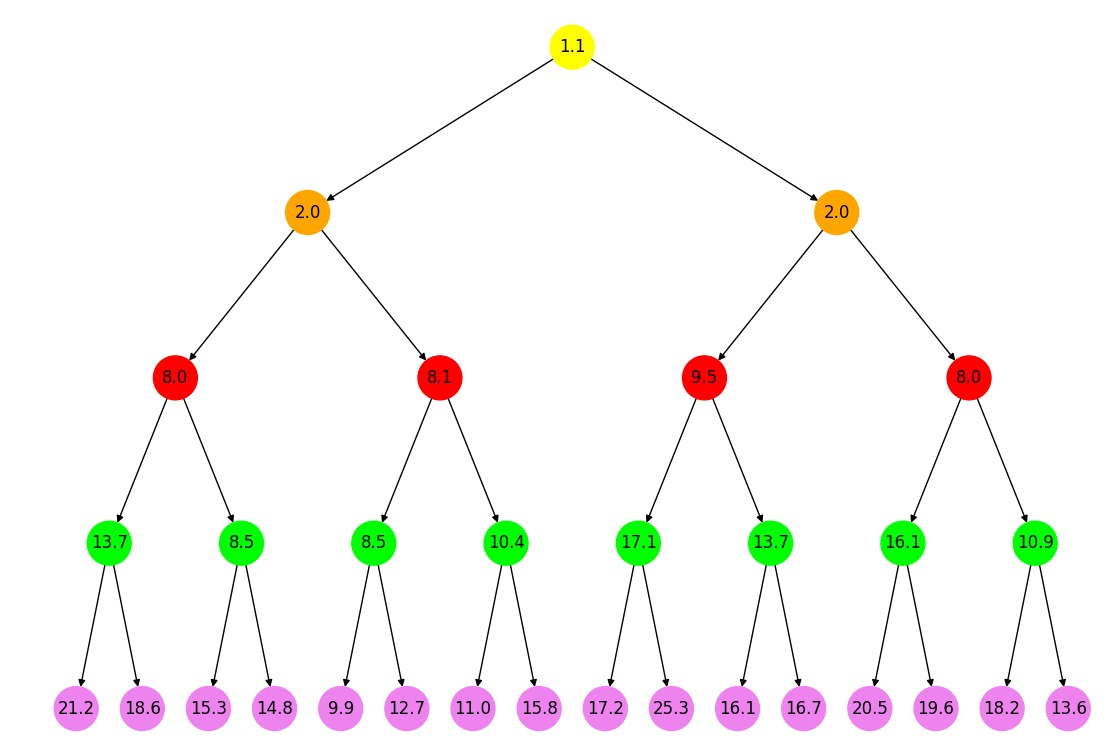
\includegraphics[width=1\linewidth]{images/algo-visualisation.jpeg}
    \caption{Visualization of heap search algorithm with n = 8}
        \label{fig:visualise}
\end{figure}
\begin{figure}
        \centering
        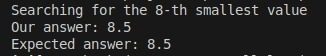
\includegraphics[width=1\linewidth]{images/algo-result.jpeg}
        \caption{Results of heap search algorithm with n = 8}
    
        \label{fig:result}
\end{figure}

\section{Complexity \& Runtime Analysis}
The theoretical complexity of the algorithm stated in the paper is $O(n\cdot \log^3(n))$. By running it, we confirm it's upper-bound. The results, normalized by division in Fig. \ref{fig:normailsed-run-time}, suggest that the results we have are a bit more optimized, and one of the reasons for that might be that we do not know the worst case and we have not tested the algorithm on the worst case, hence the discrepancy.
\begin{figure}
    \centering
    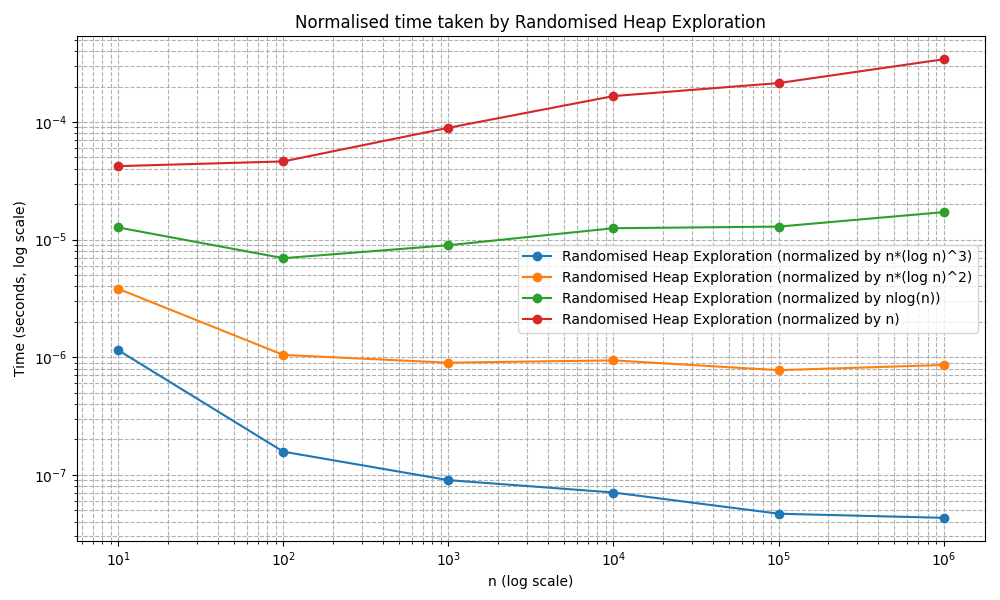
\includegraphics[width=1\linewidth]{images/normalised_performance_comparison.png}
    \caption{Normalized running times on the log-scale}
    \label{fig:normailsed-run-time}
\end{figure}
\section{Baseline or Comparative Evaluation}
We tested and compared the randomized heap search alogrithm against the baseline of best-first, and as shown in Fig. \ref{fig:comparison}, the time taken by the former is slightly higher than the latter. This is as expected since, the randomized algorithm takes up a space of $O(\log n)$ in contrast to best-first space complexity of $O(n)$. The difference is just in logarithmic factors, as seen the figure. The results produced by both matched in all instances.

\begin{figure}
    \centering
    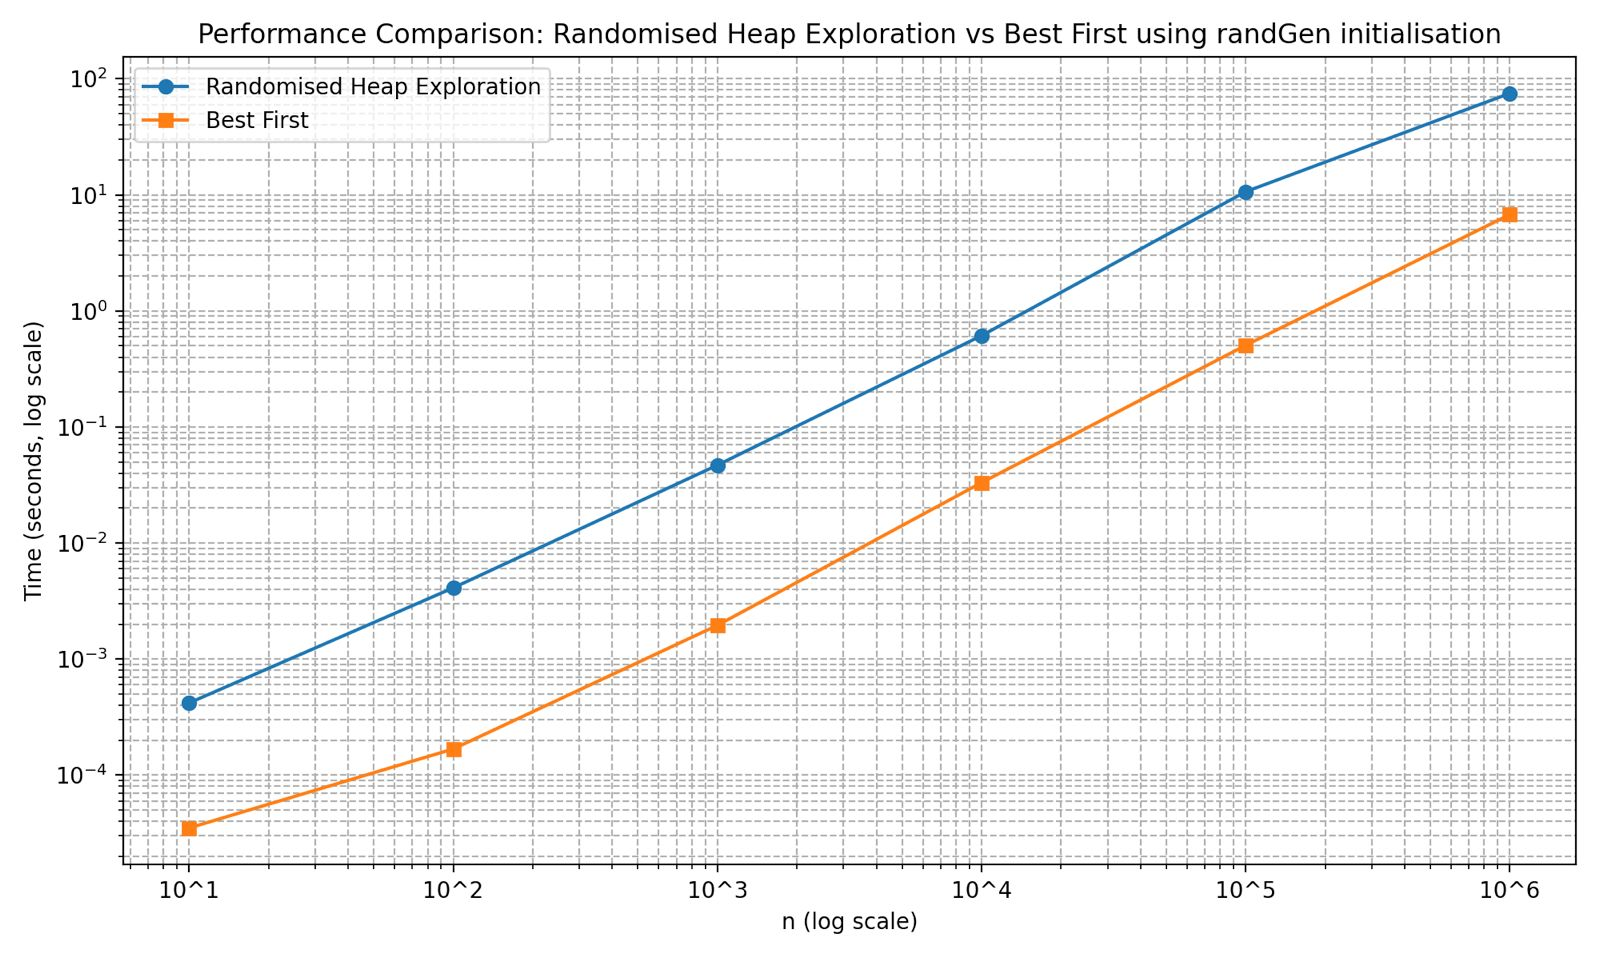
\includegraphics[width=1\linewidth]{images/algo-comparison.jpeg}
    \caption{ Baseline vs Randomized Heap Exploration}
    \label{fig:comparison}
\end{figure}

\section{Challenges \& Solutions}
\begin{enumerate}
    \item Implementing the infinite heap was an interesting problem. Breaking the heap structure down into classes and using wrapper functions for accessing children gave the idea of generating the nodes on function call, giving the impression of an infinite heap.
    \item \textsc{Roots}, \textsc{DFS}, \textsc{GoodValues} did not have pseudocode which made implementation notably harder. We resolved to reading the descriptions line by line. However, one major issue was the description of \textsc{GoodValues} seemed to have an error, which caused its randomised binary search to fail if all values were good. This was resolved by doing a check initially for the largest value.
    \item The algorithm is designed to work for heaps with distinct values. For application to knapsack, we needed support of duplicate values. For this, \textsc{DFS} had to be modified so that instead of checking there are at most $n$ values at most equal to $L$, we instead check if the $n$-th largest value is at most $L$. This is a subtle yet important difference.
    \item The description of how to use explorable heap selection for integer linear programming was not completely clear in \cite{Borst2025} so we referred to \cite{karp1986search}. However, the other paper also had a rather abstract description. To get a concrete idea, we looked into linear programming, integer linear programming (ILP), and the branch and bound method for ILP. It is a very fascinating topic, and it was really cool to see how the 0-1 Knapsack problem can be rephrased as an ILP problem.
    \item We realised that visualising the algorithm required a very deep understanding of each part of the algorithm to make a meaningful visualisation. We did try to dive deeper into the functioning of the algorithm, to determine the important steps that we could demonstrate; however, it is still far from perfect and a bit challenging to follow along, especially for those viewing the algorithm for the first time.
\end{enumerate} 

\section{Enhancements}
\begin{enumerate}
    \item We tested the algorithm on randomly generated data of our own, verifying correctness.
    \item We corrected the error in \textsc{GoodValues} subroutine.
    \item We made the algorithm work in case of repeated values in nodes.
    \item We used the algorithm for the branch and bound method to solve 0-1 Knapsack.
    \item We developed a visualization for the algorithm.
\end{enumerate}
\bibliography{references}
\bibliographystyle{plain}

\end{document}
